% Set page size and margins
% Replace `letterpaper' with `a4paper' for UK/EU standard size
\documentclass{article}

\usepackage[english]{babel}
\usepackage[a4paper,top=2cm,bottom=2cm,left=3cm,right=3cm,marginparwidth=1.75cm]{geometry}
\usepackage{times,mathptmx}
\usepackage[pdftex]{graphicx}
\usepackage{pdflscape}

\usepackage{booktabs}
\usepackage{subcaption}
\usepackage{graphicx}
\usepackage{float}
\usepackage[section]{placeins}
\usepackage{fancyhdr}
\usepackage{enumitem}
\usepackage{makecell}
\usepackage{tocloft}
\usepackage{natbib}
\usepackage[nottoc,notlof,notlot]{tocbibind} % Put the bibliography and index in the ToC

\usepackage{pifont}
\newcommand{\cmark}{\ding{51}} % ✓
\newcommand{\xmark}{\ding{55}} % ✗
\usepackage{tikz}
\usetikzlibrary{arrows.meta,positioning,shapes.geometric}
\pdfminorversion=7 %allow newer versions of .pdfs to be used as images

\pagestyle{fancy}
\rhead{}
\lhead{}
%\chead{Page \thepage}
%\cfoot{Predecisional Draft Report}
%\renewcommand{\headrulewidth}{0.4pt}
\renewcommand{\footrulewidth}{0.4pt}

\usepackage{color}
\usepackage{amsmath}
\usepackage{siunitx}
\usepackage{multirow}
\definecolor{linknavy}{rgb}{0,0,0.50196}
\definecolor{linkred}{rgb}{1,0,0}
\definecolor{linkblue}{rgb}{0,0,1}

\usepackage{xr-hyper}
\usepackage[pdftex,
colorlinks=true,
urlcolor=linkblue,     % \href{...}{...} external (URL)
citecolor=linkred,     % citation number colors
linkcolor=linknavy,    % \ref{...} and \pageref{...}
pdfproducer={pdflatex},
pagebackref,
pdfpagemode=UseNone,
bookmarksopen=true,
plainpages=false,
verbose]{hyperref}

\setlength{\textwidth}{6.5in}
\setlength{\textheight}{9.0in}
\setlength{\topmargin}{0.in}
\setlength{\headheight}{0.in}
\setlength{\headsep}{0.25in}
\setlength{\parindent}{0.25in}
\setlength{\oddsidemargin}{0.0in}
\setlength{\evensidemargin}{0.0in}




\begin{document}
	
	\bibliographystyle{unsrt}
	\thispagestyle{empty}
	
	
	\vspace*{0.75in}
	
	\begin{center}
		\begin{Large}
			{\bf Summary of Modeling Results\\ Submitted to the MaCFP-4 Condensed Phase Workshop} \\
		\end{Large}
		\hspace{1in} \\
	\end{center}
	
	\begin{center}
		\begin{large}
			Version~1.0 -- Released October 30, 2026\\
		\end{large}
		\hspace{2in} \\
	\end{center}
	
	\begin{figure}[h]
		\centering
		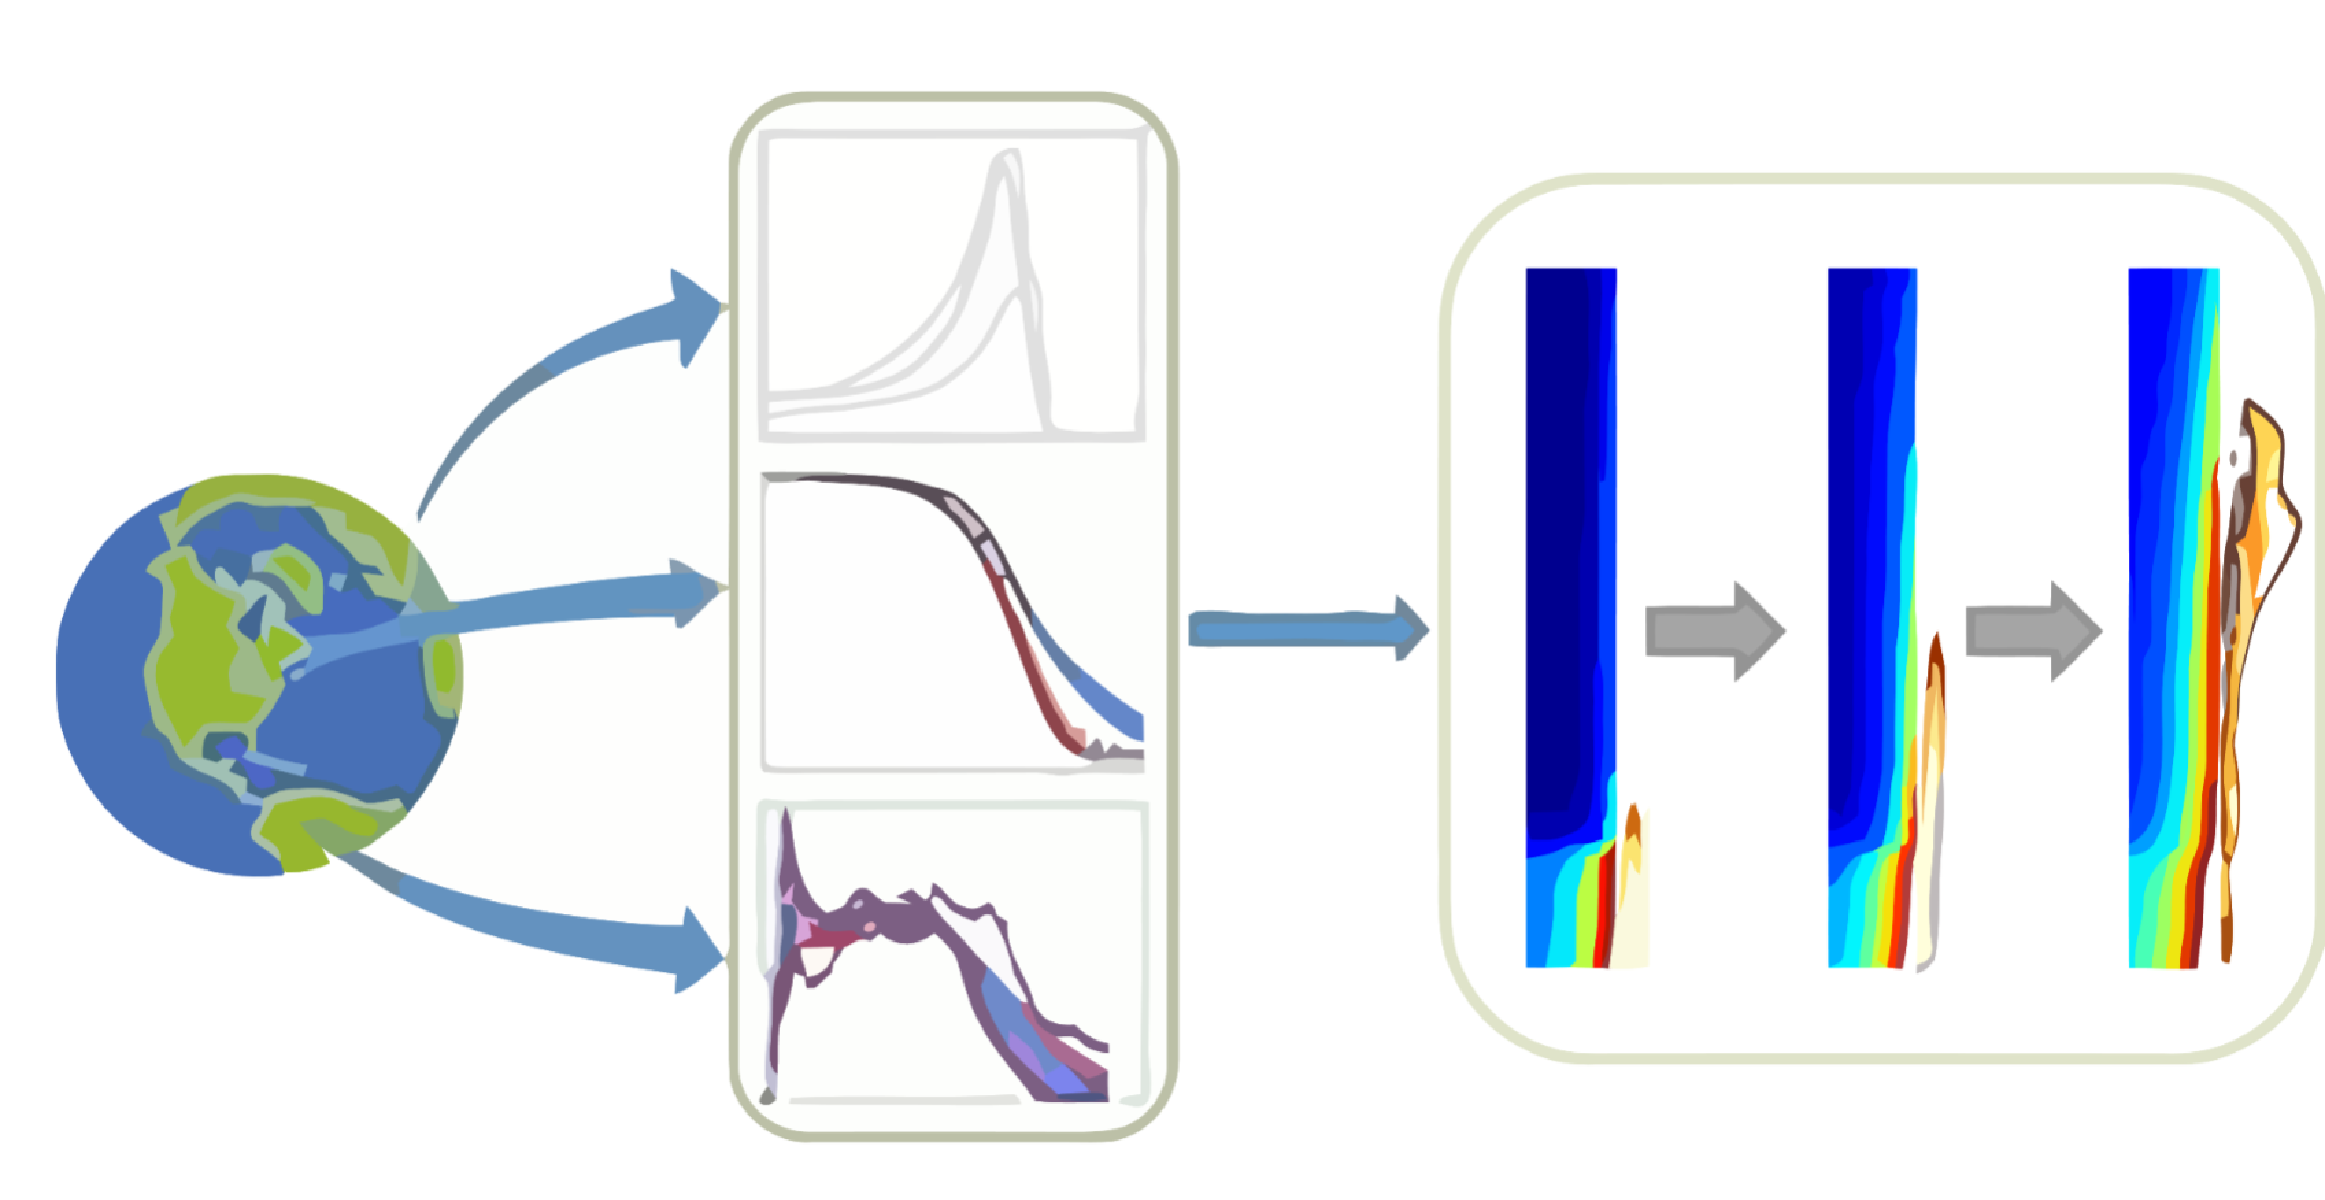
\includegraphics[width=4in]{../FIGURES/MaCFP_Logo}
		\label{Cover_Image}
	\end{figure}
	
	\vfill
	
	\begin{minipage}{0.25\textwidth}
		\begin{figure}[H]
			
\includegraphics[width=1.5in]{../FIGURES/IAFSSLogo}
		\end{figure}
	\end{minipage} \hfill
	\begin{minipage}{0.7\textwidth}
		\begin{flushright}
			%{\bf The MaCFP Condensed Phase Working Group Organizing Committee:} \\
			%Benjamin Batiot (University of Poitiers, France) \\
			%Morgan Bruns (Virginia Military Institute, USA) \\
			%Simo Hostikka (Aalto University, Finland) \\
			%Isaac Leventon (National Institute of Standards and Technology, USA) \\
			%Yuji Nakamura (Toyohashi University of Technology, Japan) \\
			%Pedro Reszka (Universidad Adolfo Ibáñez, Chile) \\
			%Thomas Rogaume (University of Poitiers, France) \\
			%Stanislav Stoliarov (University of Maryland, USA)
			\textbf{ Document Prepared by:} \\
			Abdenour Amokrane; Electricité de France (EDF)\\
			Morgan Bruns; St. Mary's University, San Antonio (StMU)\\
			Isaac Leventon; National Institute of Standards and Technology (NIST) \\
			
			\vspace{2mm}
			\textbf{Modeling Results Submitted by:}\\
			Mark McKinnon, Grayson Bellamy; UL Fire Safety Research Institute (UL FSRI) \\
			Morgan Bruns; St. Mary's University, San Antonio (StMU)\\
			Isaac Leventon; National Institute of Standards and Technology (NIST) \\
			Peter Blevington; University of Colorado Boulder (UCB)\\
			Grayson Bellamy, Stanislav Stoliarov; University of Maryland (UMD) \\ 
			
			
			
		\end{flushright}
	\end{minipage}
	
	
	\newpage
	\thispagestyle{empty}
	\pagenumbering{roman}
	
	\section*{Preface}
	\addcontentsline{toc}{section}{\protect\numberline{}Preface}
	\thispagestyle{fancy}
	This report has been prepared on behalf of the Measurement and Computation of Fire Phenomena (MaCFP) Condensed Phase Working Group. All modeling results presented here have been submitted voluntarily to the MaCFP-4 Workshop by participants of the Pyrolysis Model Calibration Exercise~\cite{MaCFP4Guidelines}. These calibrated material property sets, related predictions of material decomposition behavior (in response to idealized heating scenarios), and the corresponding meta-analysis provided in this document are presented here for subject matter experts to provide critical review and to ensure the integrity of the results submitted to the MaCFP-4 Condensed Phase Workshop. 
	
	Modelers were not provided limitations or suggestions regarding their pyrolysis model parameterization approach (i.e., material property calibration); however, they were required to use either (a) at least one of the milligram-scale datasets (e.g., TGA or DSC) and one gram-scale experiment (e.g., cone calorimetry or controlled atmosphere gasification experiments), or (b) at least two of the gram-scale experiments available in the \href{https://github.com/MaCFP/matl-db/tree/master/Wood/Calibration_Data}{Calibration\_Data section} of the MaCFP repository. A summary of the experimental measurements used for material property calibration discussed in this report is available elsewhere~\cite{MaCFP4PyrolysisExp}.

	Some material property sets presented here are incomplete (e.g., decomposition reaction mechanisms only, without associated transport properties) or offer varying degrees of accuracy with respect to experimental measurements used for property calibration. These results are welcomed submissions to the broader MaCFP effort, which seeks to foster collaborative and collegial discussions and encourages sharing of progressive, if imperfect, results to advance the community’s understanding of model performance and development. These results also enable discussion of the benefits and/or tradeoffs of using different calibration data, calibration approaches, and model complexity when developing pyrolysis property sets.
	
	Parts of this work were prepared by the National Institute of Standards and Technology (NIST), an agency of the US government, and is not subject to copyright in the USA. Not all of the measurement data presented here has been through a formal review process. The identification of any commercial product or trade name does not imply endorsement or recommendation by NIST (or any other contributing institution). The policy of NIST is to use metric units of measurement in all its publications, and to provide statements of uncertainty for all original measurements. In this document, however, data from organizations outside NIST are shown, which may include measurements in non-metric units or measurements without uncertainty statements.
	
	
	
	\newpage
%	\thispagestyle{fancy}
	\tableofcontents
	\addcontentsline{toc}{section}{\protect\numberline{}Table of Contents}
\clearpage	
	\pagenumbering{arabic}
	\pagestyle{fancy}


\section{Introduction}

The Measurement and Computation of Fire Phenomena (MaCFP) Condensed Phase Subgroup is focused on enabling the fire research community to make significant progress towards establishing a common framework for the selection of experiments (and the methodologies used to analyze these experiments) when developing pyrolysis models. Early workshops -- MaCFP-2 (2021) and MaCFP-3 (2023) -- focused on a relatively simple, non-charring material: poly(methyl methacrylate), `MaCFP-PMMA' ~\cite{MaCFP2ExpSummary, MaCFP3Proceedings}. 
The measurement data (which can be used as targets for pyrolysis model calibration and validation) and calibrated material property sets presented at MaCFP-2 and MaCFP-3 have been uniformly formatted and well-documented. This standardized data naming and formatting, as well as inclusion of corresponding metadata (describing sample preparation, test setup, and experimental conditions) allows for efficient, automated analysis. All measurements (and related analysis tools) are maintained in a digital, version-controlled, and freely-available online repository: \url{https://github.com/MaCFP/matl-db}~\cite{MaCFP-cond-db}.

For MaCFP-4, the Condensed Phase Subgroup coordinated a new $anaerobic$ pyrolysis model calibration exercise focused on pine wood. This charring material was selected based on feedback from participants of the MaCFP-3 Workshop~\cite{MaCFP3Proceedings}, a majority of whom suggested (as a critical fire modeling need) studying a new material and/or studying charring/oxidation. This specific wood species was selected because of its widespread use in construction, furnishings, and standard fire testing (e.g., crib fires). MaCFP-4 pyrolysis modeling targets included $only$ anaerobic conditions; however, participants were encouraged to develop experimental datasets and corresponding models that will describe oxidation (as will be studied in detail at MaCFP-5). The intent is that this same wood will be studied in future MaCFP modeling exercises (e.g., oxidative pyrolysis, burning, and fire growth studies).

Limited quantities of `MaCFP Wood' were sent directly~\cite{MaCFP4Guidelines} to participants who committed to conducting experiments\footnote{All `MaCFP Wood' samples -- specifically, Eastern White Pine, $Pinus Strobus$ -- were obtained from the same forest/grove in Gardners, Pennsylvania (near Pine Grove Furnace State Park in the USA). Samples were felled, dried, prepared, and cut to size for milligram- and gram-scale experiments as described elsewhere~\cite{MaCFP4PyrolysisExp}}. No single approach for pyrolysis model parameterization was  suggested to participants especially because a key objective of MaCFP-4 was to catalogue current approaches used to parameterize complex pyrolysis models. Thus, participants were encouraged to follow their best practices to enable discussion of the similarities and differences of their approaches and results (i.e., final parameterization) without explicitly requiring a final validation versus a given test. Measurement data submitted by experimentalists participating in this exercise included: milligram-scale tests (e.g., thermogravimetric analysis, TGA, differential scanning calorimetery, DSC, and microscale combustion calorimetry, MCC), gram-scale testing (e.g., gasification and cone calorimetry experiments), and 'direct' property measurements (e.g., reflectivity or thermal diffusivity). A detailed summary of these experimental measurements is available elsewhere~\cite{MaCFP4PyrolysisExp}.

Modelers were not provided limitations or suggestions regarding their pyrolysis model parameterization (i.e., calibration) approach; however, they were required to use either (a) at least one of the milligram-scale datasets and one gram-scale experiment, or (b) at least two of the gram-scale experiments available in the \href{https://github.com/MaCFP/matl-db/tree/master/Wood/Calibration_Data}{Calibration\_Data section} of the MaCFP repository. Modelers could supplement MaCFP data with any literature data that they deem necessary. Table~\ref{table:properties} lists all pyrolysis model parameters of interest (and their respective units) for this study.

\begin{table}[htb]
	\centering
	\caption{ Pyrolysis Model Parameters}
	\label{table:properties}
	\begin{tabular}{p{0.125\linewidth} | p{0.2\linewidth}| p{0.3\linewidth}}
		\hline
		\textbf{Symbol}         & \textbf{Units} & \textbf{Name}\\
		\hline
		\multicolumn{3}{c}{Degradation Kinetics}\\
		\hline
		$A$ &s$^{-1}$   &Pre-exponential constant \\
		$E$ &J mol$^{-1}$ &Activation energy \\
		$n$ &[-]    &Reaction order\\
		$\nu$ &[-]    &Stoichiometric coefficient\\
		%\multicolumn{3}{c}{**Explicitly highlight oxidation parameters?**}\\
		\hline
		\multicolumn{3}{c}{Thermodynamic Properties}\\
		\hline
		$c_p$ &J kg$^{-1}$ K$^{-1}$ &Heat capacity\\
		$h_r$ &J kg$^{-1}$    &Heat of reaction\textsuperscript{A}\\
		$\rho$  &kg m$^{-3}$    &Density\\
		\hline
		\multicolumn{3}{c}{Transport Properties}\\
		\hline
		$k$ &W m$^{-1}$ K$^{-1}$  &Thermal conductivity\\
		$D$ &m$^2$ s$^{-1}$   &Mass diffusivity\\
		$\alpha$  &m$^{-1}$ or m$^2$ kg$^{-1}$  &Absorption coefficient\\
		$\epsilon$  &[-]        &Emissivity\\
		\hline
		\multicolumn{3}{l}{\textsuperscript{A} $h_r$ reported as positive for endorthermic reactions}
	\end{tabular}
\end{table}

\pagebreak
At MaCFP-4, comparisons of pyrolysis models were made by asking modelers to use their property sets to simulate the anaerobic decomposition of `MaCFP Wood' under idealized conditions (see Fig.~\ref{fig:model-scenarios}):
\begin{enumerate}
	\item  Zero-dimensional (0D) Thermogravimetric Analysis (TGA) and Differential Scanning Calorimetry (DSC) experiments conducted at two constant heating rates (10~K/min and 100~K/min); and
	\item One-dimensional (1D), radiation-driven gasification scenarios conducted at three incident radiant heat fluxes (10~kW/m$^2 \leq q^{''}_{rad} \leq 60$~kW/m$^2$; no convection, adiabatic back surface) and two thicknesses (6~mm and 18~mm).
\end{enumerate}

\begin{figure}[h!]
	\centering
	
	\begin{subfigure}[t]{0.35\textwidth}
		\centering
		\includegraphics[width=\textwidth, trim=6 6 6 6, clip]{../FIGURES/MaCFP4/model-TGA.pdf}
		\label{Fig:model-TGA}
		\caption{}
	\end{subfigure}
	\hspace{0.1\textwidth}
	\begin{subfigure}[t]{0.35\textwidth}
		\centering
		\includegraphics[width=\textwidth, trim=6 6 6 6, clip]{../FIGURES/MaCFP4/model-gasification.pdf}
		\label{Fig:model-gasification}
		\caption{}
	\end{subfigure}
	
	\caption{Schematics of idealized (a) 0D and (b) 1D heating scenarios considered in model-to-model comparisons of idealized thermal decomposition of `MaCFP-Wood'.}
	\label{fig:model-scenarios}
\end{figure}

In the case of the TGA simulations, mass loss rate profiles as a function of temperature were used for comparison. In the case of the DSC simulations, temperature-resolved heat flow rate and integral heat flow profiles will be used for comparison. In the case of the gasification simulations, mass loss rate and surface temperature profiles will be used for comparison. A summary of pyrolysis model comparison conditions and target outputs is provided in Table~\ref{table:Pyrolsis Model Comparison}.

\begin{table}[t!]
	\centering
	\caption{Pyrolysis Model Comparison Conditions}
	\label{table:Pyrolsis Model Comparison}
	\begin{tabular}{p{0.25\linewidth} p{0.6\linewidth}}
		\hline
		\multicolumn{2}{c}{\textbf{Thermogravimetric Analysis (TGA) Experiments} \quad [Two simulations]}\\
		\multicolumn{2}{c}{\textbf{Differential Scanning Calorimetry (DSC) Experiments} \quad [Two simulations]}\\
		\hline
		Temperature Range: & 300~K to 1000~K\\
		Heating Rates: & 10 K min\textsuperscript{-1} and 100 K min\textsuperscript{-1}\\
		Initial Sample Mass & 5 mg\\
		Output: & time [s]\\
		& Time-resolved Sample Temperature [K]\\
		& Time-resolved Sample Mass [mg]\\
		& Time-resolved heat flow [mW/mg]\\
		Test Description: & Simulations of idealized TGA/DSC experiments in which sample temperature must remain spatially uniform.\\
		\\
		\hline
		\multicolumn{2}{c}{\textbf{Idealized Gasification Experiments}\quad [Six simulations]}\\
		\multicolumn{2}{c}{Simulations should be performed using a computational pyrolysis solver.}\\
		\hline
		Initial Temperature: & Initial ambient and sample temperatures should be 293~K\\
		Top Boundary:& Sample surface exposed to 10, 30, and 60~kW~m$^{-2}$ of\\
		& incident radiant heat flux; no convection\\
		Bottom Boundary: & Sample back surface should be perfectly insulated \\
		& (i.e., no convection or radiation)\\
		Sample Dimensions: & Simulations should be repeated at each incident heat flux using sample thicknesses of 6~mm and 18~mm
		Simulation outputs should be scaled such that samples are initial 10~cm~x~10~cm, squares.\\
		Output: & Time [s]\\
		& Time-resolved Sample Mass [g]\\
		& Time-resolved Sample Back-Surface Temperature [K]\\
		& Time-resolved Sample Top-Surface Temperature [K]\\
		\hline
	\end{tabular}
\end{table}



To perform this phase of the modeling exercise, participants required input data in the form of kinetic parameters and thermophysical properties. Modelers were free to use experimental data generated by any participant in the associated experimental benchmark exercise~\cite{MaCFP4PyrolysisExp}, to perform their own parameter calibrations, or to adopt a combination of both approaches (or even complete the data set from literature). It should be noted that the calibration of kinetic and thermophysical parameters constituted an integral part of the benchmark exercise, thus the resulting methodologies and outcomes are discussed separately in this report.

\clearpage
\section{Participating organizations}

A total of ten different material property sets were received from six participating institutions (see Table~\ref{tab:pyrolysis-conributors}). Two of these submissions resulted from collaborations between two organizations. All organizations simulated the full set of scenarios, except NIST-StMU, which submitted simulations for the OD scenarios only (i.e., TGA and DSC). 


\begin{table}[htbp]
	\centering
	\small
	\caption{Contributors to the Pyrolysis Model Calibration Exercise} \label{tab:pyrolysis-conributors}
	\begin{tabular}{@{}p{7cm}p{4cm}p{4cm}@{}}
				\hline
		\textbf{Institution} & \textbf{Location} & \textbf{Modeling} \\
		\hline
		Complexe de Recherche Interprofessionnel en Aérothermochimie (CORIA)& Rouen, France & TGA, Gasification \\
		National Institute of Standards and Technology (NIST) & Maryland, USA & TGA, DSC\\
		Saint Mary's University, San Antonio (StMU) & Texas, USA & TGA, DSC\\
		University of Colorado, Boulder (UCB) & Colorado, USA & TGA, DSC, Gasification (6~approaches) \\
		UL Fire Safety Research Institute (UL FSRI) & Maryland, USA & TGA, DSC, Gasification (2~approaches) \\
		University of Maryland (UMD) & Maryland, USA & STA, Gasification \\
		
		\hline
	\end{tabular}
	\normalsize
\end{table}

%Table~\ref{tab:organization_scenarios} summarizes the scenarios modelled by the participating organizations. .

%\begin{table}
%\centering
%\begin{tabular}{c|c|c|c|c}
%                & \textbf{CORIA}         & \textbf{FSRI - UMD} & NIST-StMU  & UCB     \\\hline
%\textbf{0D TGA} & \cmark                 & \cmark              & \cmark     & \cmark  \\
%\textbf{1D FPA} & \cmark                 & \cmark              & \xmark     & \cmark
%\end{tabular}
%\caption{\label{tab:organization_scenarios}Simulated scenarios by the participating organizations.}
%\end{table}

\section{Model Development}
This section provides a brief description of the physical assumptions adopted by the different participating organizations when developing their respective models. Further information is provided in the Supplemental Information Section of this report (Sec.~\ref{sec:SI}).

\subsection{CORIA modeling assumptions}

The pyrolysis process was represented by three parallel decomposition reactions corresponding to the three main wood pseudo-components (nominally hemicellulose, cellulose, and lignin, see eqn.~\ref{eq:CORIA-pyrolysis-reactions}). The initial mass fraction of these pseudo-components, are taken from literature \cite{marquez2021kinetic}: 0.163, 0.544 and 0.293, respectively. Dry wood was assumed in both the OD and 1D simulations. The kinetic parameters were identified from TGA experiments from the MaCFP-4 experimental database (\href{https://github.com/MaCFP/matl-db/tree/master/Wood/Calibration_Data/UMET}{UMET data set}), using the DAKOTA code and the NL2SOL optimization algorithm, and the resulting kinetic mechanism was subsequently employed in the 0D and 1D simulations. Constant thermophysical properties, taken from the literature (Dinh PhD Dissertation~\cite{dinh2024developpement}), were considered throughout the simulations. For the 1D configuration, fibers were assumed to be oriented perpendicular to the exposed surface. The gasification simulations were performed with the PATO code \cite{lachaud2017generic}. Radiative heat exchange was prescribed at the exposed surface, with no convection. A zero-temperature-gradient condition was imposed at the rear surface.

\begin{equation}
\label{eq:CORIA-pyrolysis-reactions}
\begin{aligned}
\mathrm{Cellulose}      &\rightarrow n_1\,\mathrm{char} + (1-n_1)\,\mathrm{gas} \\
\mathrm{Hemicellulose}  &\rightarrow n_2\,\mathrm{char} + (1-n_2)\,\mathrm{gas} \\
\mathrm{Lignin}         &\rightarrow n_3\,\mathrm{char} + (1-n_3)\,\mathrm{gas}
\end{aligned}
\end{equation}

%\begin{figure}
%\centering
%\includegraphics[width=0.25\linewidth]{frog.jpg}
%\caption{\label{fig:frog}This frog was uploaded via the file-tree menu.}
%\end{figure}


\subsection{FSRI - UMD modeling assumptions}
The FSRI-UMD collaboration submitted two distinct models (i.e., two material property sets):
\begin{itemize}
	\item (\textbf{FSRI-UMD OPT}): an optimized property set, relying primarily on inverse analysis
	\item (\textbf{FSRI-UMD DM}): based as much as possible on directly measured properties	
\end{itemize}
Temperature-dependent thermophysical properties were considered throughout the simulations. \\

Both OPT and DM models employed the same thermal degradation kinetics and thermodynamics. The pyrolysis process was represented by six sequential first-order reactions, including one moisture evaporation reaction and five thermal degradation reactions\footnote{For the 1D Idealized Gasification simulations, the models were implemented in FDS version 6.10.1, neglecting the moisture evaporation reaction.}. Kinetic and energetic parameters were calibrated against STA (i.e., combined TGA and DSC) measurements obtained at multiple heating rates. The kinetic parameters were identified from STA experiments conducted by FSRI at 3~K~min$^{-1}$ and 30~K~min$^{-1}$ and by UMD at 10~K~min$^{-1}$ using a multi-stage hill-climbing optimization algorithm implemented in Julia and coupled with the \texttt{Pyrolysis.jl} model. 


Temperature-dependent specific heat capacities of the virgin material were determined through a linear interpolation of `directly measured' specific heat capacities (heat flow meter measurements between 25$^\circ$C and 45$^\circ$C) and apparent specific heat capacity (DSC measurements obtained between 150$^\circ$C and 185$^\circ$C; $\frac{dT}{dt}=10$~K/min). Char heat capacity was determined by fitting DSC data above the endset temperature of decomposition (STA experiments $\frac{dT}{dt}=10$~K/min).

In the FSRI-UMD OPT model, the heat capacities of intermediate species were fit as weighted averages of apparent specific heat capacities of virgin wood and char. Char and Ash were defined to share the same linear form. Moisture specific heat capacity taken from the NIST Chemistry Webbook~\cite{linstrom2001nist}. The heats of reaction were subsequently calibrated against DSC measurements acquired at 10 K min$^{-1}$. The FSRI-UMD OPT model also incorporated a state-dependent heat of sorption function that relies on temperature and moisture content. 

Density of the dried virgin component was determined from direct mass and volume measurements of regular shaped samples. The density of solid products of decomposition were determined from a combination of TGA and dilatometry data (both at 10K/min) for both models.
Surface emissivities were based on integrating-sphere measurements and depended on the incident heat flux. FTIR Integrating Sphere measurements were repeated on both virgin wood and char; emissitivities of intermediate species were assumed to be either (1) equal to one of these two values, or (2) equal to a weighted fraction of these two values. For both models, the absorption coefficient was assumed to be sufficiently high that all radiation was absorbed at the boundary. 

\subsection{NIST-StMU modeling assumptions}

The material property set submitted by NIST-StMU was calibrated using a hierarchical approach in which material properties are uniquely calibrated from individual measurements/datasets. For MaCFP-4, the NIST-StMU group provided a material property set based on the following measurements:
\begin{itemize}
	\item Thermogravimetric Analysis (TGA): Decomposition reaction mechanism (\textcolor{red}{3**} parallel reactions), kinetics
	\item Differential Scanning Calorimetry (DSC): Heat capacities, Heats of reaction
	\item Microscale Combustion Calorimeter (MCC): Heats of combustion (flaming & charring) 
	\item  FTIR + Integrating Sphere: reflectivity
\end{itemize}

The decomposition process was represented by three parallel reactions corresponding to the decomposition of the main wood constituents (moisture loss is neglected). Constant thermophysical properties were assumed throughout the simulations though unique specific heat capacities were prescribed for the virgin wood and the char. Property calibration was performed using Flammability data Automated Calibration Tools (FACT), which are a suite of automated Python scripts for estimating material properties from small scale tests.
 NIST-StMU properties were only used to predict 0D decomposition (i.e., idealized TGA/DSC tests) for the model-to-model comparison exercise.

\subsection{UCB modeling assumptions}
UCB submitted 12 distinct models (i.e., 12 material property sets). Each model used (1) one of three reaction schemes, (2) either constant or temperature-dependent material properties, and (3) thermophysical/transport properties calibrated to describe samples in which wood grains are oriented either parallel or perpendicular to the front surface of the wood. Each reaction scheme assumed that wood consisted of three main constituents -- cellulose, hemicellulose, and lignin -- each of which can decompose in parallel. 

The three reaction schemes ranged from a simple three-reaction, parallel mechanism to more detailed, component-wise, multi-step reaction schemes. For each scheme, individual char species may be lumped together by giving them identical material properties. A brief description of these reaction schemes is provided below; more information is \href{https://github.com/MaCFP/matl-db/tree/master/Wood/Calibration_Results/UCB#readme}{available elsewhere}:.
\begin{itemize}
	\item Reaction scheme 1 (eqn.~\ref{eq:UCB1}): Single-stage, parallel reaction mechanism whereby individual components are each converted to char through one of three parallel reactions. Here, 6 total species are tracked, as each reaction produces a different char residue. 
	\item Reaction scheme 2 (eqn.~\ref{eq:UCB2}): multi-stage, parallel reaction mechanism whereby individual components are likewise converted to intermediate solid species, which are then converted to char residue through another set of parallel reactions. This gives a total of 6 reactions and 9 species
	\item Reaction scheme 3 (eqn.~\ref{eq:UCB3}): Unique reaction mechanisms for each individual component, based on TGA mass loss curves for each component measured in Ref.~\cite{hasburgh2020chemical}. The best reaction scheme for each component was found through trial and error: cellulose: 2-step serial, hemicellulose: 3-step serial, and lignin: 2-step parallel. These individual component reaction schemes are combined in parallel to form the overall reaction scheme for wood, consisting of 11 species and 8 reactions. 
\end{itemize}
 Kinetic parameters for each reaction scheme were identified from TGA measurements using the gpyro v0.8200 code coupled with the Shuffled Complex Evolution (SCE) optimization algorithm. The initial mass fractions of cellulose, hemicellulose, and lignin were first estimated from component-specific TGA data and subsequently used in the kinetic calibration. 

One-dimensional gasification simulations were performed using a modified OpenFOAM solver, porousFireDyMFoam, based on the gpyro biomass pyrolysis model. Thermophysical properties were calibrated against available gasification experiments. Both constant and temperature-dependent material properties were considered. Simulations were conducted for both parallel and perpendicular grain orientations. Property estimation for the gasification simulations was carried out using the Dakota optimization framework coupled to the one-dimensional model.

\begin{equation}
\label{eq:UCB1}
\left.
\begin{aligned}
&\textbf{Cellulose:}
%\left\{
\begin{aligned}
\mathrm{~Cellulose}
&\rightarrow
\nu_1\,\mathrm{char}_1
+
(1-\nu_1)\,\mathrm{gas}
\end{aligned}
%\right.
\\[8pt]
&\textbf{Hemicellulose:}
%\left\{
\begin{aligned}
\mathrm{~Hemicellulose}
&\rightarrow
\nu_2\,\mathrm{char}_2
+
(1-\nu_2)\,\mathrm{gas}
\end{aligned}
%\right.
\\[8pt]
&\textbf{Lignin:}
%\left\{
\begin{aligned}
\mathrm{~Lignin}
&\rightarrow
\nu_3\,\mathrm{char}_3
+
(1-\nu_3)\,\mathrm{gas}
\end{aligned}
%\right.
\end{aligned}
\right\}
\end{equation}

%%%%% UCB2
\begin{equation}
\label{eq:UCB2}
\left.
\begin{aligned}
&\textbf{Cellulose:}
\left\{
\begin{aligned}
\mathrm{Cellulose}
&\rightarrow
\nu_1\,\mathrm{int}_1
+
(1-\nu_1)\,\mathrm{gas}
\\
\mathrm{int}_1
&\rightarrow
\nu_4\,\mathrm{char}_1
+
(1-\nu_4)\,\mathrm{gas}
\end{aligned}
\right.
\\[12pt]
&\textbf{Hemicellulose:}
\left\{
\begin{aligned}
\mathrm{Hemicellulose}
&\rightarrow
\nu_2\,\mathrm{int}_2
+
(1-\nu_2)\,\mathrm{gas}
\\
\mathrm{int}_2
&\rightarrow
\nu_5\,\mathrm{char}_2
+
(1-\nu_5)\,\mathrm{gas}
\end{aligned}
\right.
\\[12pt]
&\textbf{Lignin:}
\left\{
\begin{aligned}
\mathrm{Lignin}
&\rightarrow
\nu_3\,\mathrm{int}_3
+
(1-\nu_3)\,\mathrm{gas}
\\
\mathrm{int}_3
&\rightarrow
\nu_6\,\mathrm{char}_3
+
(1-\nu_6)\,\mathrm{gas}
\end{aligned}
\right.
\end{aligned}
\right\}
\end{equation}

% UCB3
\begin{equation}
\label{eq:UCB3}
\left.
\begin{aligned}
&\textbf{Cellulose:}
\left\{
\begin{aligned}
\mathrm{Cellulose} &\rightarrow \nu_1\,\mathrm{int}_1 +(1-\nu_1)\,\mathrm{gas} \\
\mathrm{int}_1 &\rightarrow \nu_2\,\mathrm{char}_1 +(1-\nu_2)\,\mathrm{gas}
\end{aligned}
\right.
\\[10pt]
&\textbf{Hemicellulose:}
\left\{
\begin{aligned}
\mathrm{Hemicellulose} &\rightarrow \nu_3\,\mathrm{int}_2 +(1-\nu_3)\,\mathrm{gas} \\
\mathrm{int}_2 &\rightarrow \nu_4\,\mathrm{int}_3 +(1-\nu_4)\,\mathrm{gas} \\
\mathrm{int}_3 &\rightarrow \nu_5\,\mathrm{char}_2 +(1-\nu_5)\,\mathrm{gas}
\end{aligned}
\right.
\\[10pt]
&\textbf{Lignin:}
\left\{
\begin{aligned}
\mathrm{Lignin} &\rightarrow \nu_6\,\mathrm{char}_3 +(1-\nu_6)\,\mathrm{gas} \\
\mathrm{Lignin} &\rightarrow \nu_7\,\mathrm{int}_4 +(1-\nu_7)\,\mathrm{gas} \\
\mathrm{int}_4 &\rightarrow \nu_8\,\mathrm{char}_4 +(1-\nu_8)\,\mathrm{gas}
\end{aligned}
\right.
\end{aligned}
\right\}
\end{equation}
\\
By combining the different modelling assumptions, the UCB contribution resulted in three models for each 0D decomposition case, corresponding to the three reaction mechanisms described above. For the idealized 1D gasification simulations, the combination of the three reaction mechanisms, two thermophysical property formulations (constant and temperature-dependent), and two grain orientations (parallel and perpendicular) led to a total of twelve models for each gasification case. To facilitate the discussion of the results, the naming convention illustrated in Fig.~\ref{fig:ucb-naming} was adopted throughout this report.

\begin{figure}[htbp]
\centering
\begin{tikzpicture}[>=stealth]

% Texte principal
\node (ucb) at (0,0) {\Large \textbf{UCB PL-TDEP-3}};

% Ellipse autour de PL
\node[draw,ellipse,minimum width=0.9cm,minimum height=0.7cm]
(pl) at (-0.4,0) {};

% Ellipse autour de TDEP
\node[draw,ellipse,minimum width=1.7cm,minimum height=1.0cm]
(tdep) at (0.9,0) {};

% Ellipse autour de 3
\node[draw,ellipse,minimum width=0.7cm,minimum height=0.7cm]
(scheme) at (2.2,0) {};

% Boîte du haut
\node[
draw,
rectangle,
minimum width=4.5cm,
minimum height=1cm,
align=center
] (top) at (1.2,2.5)
{Temperature-dependent (\textbf{TDEP}) or \\ constant (\textbf{CONST}) properties};

% Boîte bas gauche
\node[
draw,
rectangle,
minimum width=4cm,
minimum height=1cm,
align=center
] (leftbox) at (-3,-2.2)
{Parallel (\textbf{PL}) or perpondicular (\textbf{PD})\\ grain orientation};

% Boîte bas droite
\node[
draw,
rectangle,
minimum width=4cm,
minimum height=1cm,
align=center
] (rightbox) at (4,-2.2)
{Reaction scheme (\textbf{1, 2 or 3})};

% Flèches
\draw[->] (pl.south) -- (leftbox.north);
\draw[->] (tdep.north) -- (top.south);
\draw[->] (scheme.south) -- (rightbox.north);

\end{tikzpicture}
\caption{Interpretation of the naming convention UCB-PL-TDEP-3.}
\label{fig:ucb-naming}
\end{figure}

\section{Property Comparison}
\textcolor{red}{
\textbf{Kinetics}\\
\textbf{Heat capacity}\\
\textbf{Heat of Reaction}\\
\textbf{Density}\\
\textbf{Conductivity}\\
\textbf{Radiation Properties}\\
}
\section{Model-to-Model Comparison}

The objective of the MaCFP-4 condensed-phase benchmark exercise is to perform a model-to-model comparison. Since no common set of physical assumptions was imposed on the participants, and considering the diversity of the submitted modelling approaches, each contribution was treated as a separate model in the analysis. This approach makes it possible to assess the extent to which different modelling choices and assumptions affect the predicted results. Furthermore, the comparison of these contributions provides an opportunity to evaluate the individual influence of specific modelling assumptions on the simulation outcomes.

\subsection{TGA results}
The TGA results are evaluated based on two criteria: (i) the comparison of the mass loss rate (MLR) curves and (ii) the comparison of the peak MLR (\textbf{pMLR}) values together with their corresponding temperatures(\textbf{T\_pMLR}). The analysis is conducted for two simulated heating rates, 10 K/min and 100 K/min.\\

To compare the mass loss rate (MLR) predictions, the mass loss curves provided by the participating organizations were first differentiated to obtain the corresponding MLR curves. The resulting MLR data were then interpolated onto a common grid, enabling the calculation of the mean value (Eq. \ref{eq:mean_value}) and the standard deviation (Eq. \ref{eq:std_deviation}) at each point. In these equations, $x_i$ denotes the predicted value at a given time, $n$ is the number of predictions, $\bar{x}$ (or $Mean$) represents the mean value, and $Std$ denotes the standard deviation. The purpose of calculating the mean value and its associated standard deviation is to quantify the degree of agreement among the different model predictions. A low standard deviation indicates a strong consistency between the models, whereas a high standard deviation reflects a greater spread in the predictions and, therefore, a lower level of agreement among the participants.

\begin{equation} 
\bar{x} = \frac{1}{n}\sum_{i=1}^{n} x_i 
\label{eq:mean_value}
\end{equation}

\begin{equation} 
Std = \sqrt{ \frac{\sum_{i=1}^{n}\left(x_i-\bar{x}\right)^2} {n-1} } 
\label{eq:std_deviation}
\end{equation}

Figures \ref{fig:TGA_10K/min} and \ref{fig:TGA_100K/min} present the TGA mass loss rate (MLR) curves obtained for heating rates of 10 K/min and 100 K/min, respectively. The predictions for the 10 K/min case exhibit substantial discrepancies, with peak MLR values differing by up to one order of magnitude. Nevertheless, most predictions remain clustered within a relatively narrow range, while one contribution clearly deviates from the others, likely as a result of an error in the submitted data. To enable a more meaningful comparison, the 10 K/min analysis was repeated without this outlying contribution (Figure \ref{fig:TGA_100K/min_withoutFSRI}).

Excluding this dataset reveals an improved level of agreement among the remaining predictions, although noticeable differences still persist. These discrepancies may arise from the different modelling assumptions adopted by the participants, as well as from the experimental datasets selected for model calibration. Indeed, the experimental benchmark exercise, which included both TGA and gasification measurements, highlighted considerable variability among the submitted experimental results. Since the present modelling exercise relies directly on these experimental data, part of the observed variability in the predictions can reasonably be attributed to the variability already present in the benchmark measurements themselves.

The results obtained for the 100 K/min heating rate exhibit even larger discrepancies among the different contributions. The predicted peak MLR values vary by nearly a factor of two between the lowest and highest predictions. This behaviour may be explained by the same two factors discussed previously, namely differences in modelling assumptions and differences in the experimental datasets used for model calibration. It is also worth noting that the discrepancies observed in the experimental benchmark data become more pronounced at higher heating rates. Since the present modelling exercise is directly based on these experimental measurements, part of the variability observed in the predictions at 100 K/min is likely inherited from the increased uncertainty and scatter in the underlying experimental data. 

\begin{figure}[htbp]
    \centering
    \includegraphics[width=0.8\textwidth]{TGA_figures/TGA_10K-min.png}
    \caption{Predicted TGA MLR at 10 K/min.}
    \label{fig:TGA_10K/min}
\end{figure}

\begin{figure}[htbp]
    \centering
    \includegraphics[width=0.8\textwidth]{TGA_figures/TGA_100K-min.png}
    \caption{Predicted TGA MLR at 100 K/min.}
    \label{fig:TGA_100K/min}
\end{figure}

\begin{figure}[htbp]
    \centering
    \includegraphics[width=0.8\textwidth]{TGA_figures/TGA_10K-min_withoutFSRI.png}
    \caption{Predicted TGA MLR at 10 K/min (reproduction of Figure \ref{fig:TGA_10K/min} excluding singular behavior shown by one contribution).}
    \label{fig:TGA_100K/min_withoutFSRI}
\end{figure}

Table \ref{tab:TGA_stats} summarizes the mean values and standard deviations of the predicted peak mass loss rates (pMLR) and the corresponding peak temperatures. An interesting observation is that all participants predicted very similar temperatures at peak MLR, with a standard deviation of less than 1\% for both heating rates. In contrast, the variability in the predicted pMLR values is much larger, particularly for the 10 K/min case.

This high standard deviation at 10 K/min is primarily driven by the singular behaviour of one contribution discussed previously. When this outlying prediction is excluded from the analysis, the standard deviation of the pMLR decreases significantly, indicating a better agreement among the remaining contributions.

Overall, these results are encouraging, especially considering the complexity of the material behaviour and the significant scatter observed in the experimental data used as the basis for model calibration. The close agreement in the predicted peak temperatures, together with the improved consistency in pMLR predictions after removal of the apparent outlier, suggests that the participating models capture the main features of the thermal degradation process in a relatively consistent manner.  

\begin{table}[htbp] 
\centering 
\caption{Statistical summary of the predicted TGA peak mass loss rate (pMLR) and corresponding temperature.} 
\label{tab:TGA_stats} 
\begin{tabular}{lcccc} 
\toprule & \multicolumn{2}{c}{10 K/min} & \multicolumn{2}{c}{100 K/min} \\ \cmidrule(lr){2-3} \cmidrule(lr){4-5} & pMLR (g/s) & $T_{\mathrm{pMLR}}$ (K) & pMLR (g/s) & $T_{\mathrm{pMLR}}$ (K) \\ 
\midrule 
Mean value & 0.014 & 635 & 0.061 & 685 \\ 
Standard deviation (\%) & 121 & 1 & 23 & 1 \\ \bottomrule 
\end{tabular} 
\end{table}

\subsection{Gasification results (FPA simulations)}

The 1D gasification results are evaluated using the following two approaches: 
\begin{enumerate} 
\item Comparison of the mass loss rate (MLR) and back-surface temperature curves. 
\item Comparison of key characteristic quantities, namely the peak mass loss rate ($pMLR$), the time to peak mass loss rate ($t_{\mathrm{pMLR}}$), the onset time ($t_{\mathrm{onset}}$), and the end-of-pyrolysis time ($t_{\mathrm{end}}$). \end{enumerate} 

The analysis is performed for six simulation scenarios, corresponding to the combination of three external heat fluxes (10, 30, and 60~kW\,m$^{-2}$) and two sample thicknesses (6 and 18~mm). As discussed above, the various contributions provided by the participating organizations are considered as independent model predictions because they are based on different modelling assumptions, parameter sets, and calibration strategies. As a result, the present comparison comprises one model from CORIA, two models from UMD-FSRI, and twelve models from UCB.\\

Figures \ref{fig:FPA_MLR_q10_6mm} to \ref{fig:FPA_MLR_q60_18mm} present the predicted mass loss rate (MLR) curves for the different heat fluxes and sample thicknesses considered in this study. For each case, the ensemble mean prediction is shown together with a shaded region representing the standard deviation. 

Overall, the different models exhibit a consistent qualitative behaviour. At low heat fluxes, the predictions generally display a single dominant MLR peak, whereas a more pronounced double-peak behaviour emerges as the incident heat flux increases. This trend is observed for most contributions and is therefore reflected in the mean predictions. Since oxidation processes are not considered in the present simulations, the appearance of two distinct peaks cannot be attributed to char oxidation. Instead, it is likely related to the thermal decomposition of the different wood constituents and the development of temperature gradients within the sample. Hemicellulose typically decomposes at lower temperatures than cellulose, while lignin degrades over a much broader temperature range. As the heat flux increases, the heating rate becomes higher and these degradation stages may become more clearly separated in time, leading to the emergence of two distinct MLR peaks. In addition, the larger temperature gradients that develop within the material under higher thermal loads, together with the formation of a char layer at the surface, can further promote the separation of the dominant decomposition processes. The models also successfully predict an increase in the peak mass loss rate (MLR) and a reduction in fire duration with increasing heat flux. Conversely, increasing the material thickness is predicted to decrease the peak MLR while extending the fire duration.

\begin{figure}[htbp]
    \centering
    \includegraphics[width=0.8\textwidth]{FPA_figures/mlr_vs_t_q10_6mm.png}
    \caption{Predicted 1D gasification MLR: heat flux = 10 kW/m²; thickness = 6mm.}
    \label{fig:FPA_MLR_q10_6mm}
\end{figure}
\begin{figure}[htbp]
    \centering
    \includegraphics[width=0.8\textwidth]{FPA_figures/mlr_vs_t_q10_18mm.png}
    \caption{Predicted 1D gasification MLR: heat flux = 10 kW/m²; thickness = 18mm.}
    \label{fig:FPA_MLR_q10_18mm}
\end{figure}
\begin{figure}[htbp]
    \centering
    \includegraphics[width=0.8\textwidth]{FPA_figures/mlr_vs_t_q30_6mm.png}
    \caption{Predicted 1D gasification MLR: heat flux = 30 kW/m²; thickness = 6mm.}
    \label{fig:FPA_MLR_q30_6mm}
\end{figure}
\begin{figure}[htbp]
    \centering
    \includegraphics[width=0.8\textwidth]{FPA_figures/mlr_vs_t_q30_18mm.png}
    \caption{Predicted 1D gasification MLR: heat flux = 30 kW/m²; thickness = 18mm.}
    \label{fig:FPA_MLR_q30_18mm}
\end{figure}
\begin{figure}[htbp]
    \centering
    \includegraphics[width=0.8\textwidth]{FPA_figures/mlr_vs_t_q60_6mm.png}
    \caption{Predicted 1D gasification MLR: heat flux = 60 kW/m²; thickness = 6mm.}
    \label{fig:FPA_MLR_q60_6mm}
\end{figure}
\begin{figure}[htbp]
    \centering
    \includegraphics[width=0.8\textwidth]{FPA_figures/mlr_vs_t_q60_18mm.png}
    \caption{Predicted 1D gasification MLR: heat flux = 60 kW/m²; thickness = 18mm.}
    \label{fig:FPA_MLR_q60_18mm}
\end{figure}

Figures \ref{fig:FPA_Tback_q10_6mm} to \ref{fig:FPA_MLR_q60_18mm} present the back-surface temperature predicted by the different models under the various operating conditions. Similar to the mass loss rate (MLR) results, all models predict the same general trends. Specifically, the models predict an increase in the asymptotic back-surface temperature with increasing heat flux, accompanied by a shorter transient phase. Conversely, increasing the sample thickness results in a lower asymptotic temperature and a longer transient phase before steady-state conditions are reached. It is also worth noting that the models tend to produce more consistent predictions during the steady-state phase than during the transient phase. Another interesting observation is the overall better agreement between the models for the thinner samples compared to the thicker ones. A possible explanation is that increasing the sample thickness results in the formation of a thicker char layer, which enhances the influence of physical phenomena such as radiative heat transfer and mass transport within the porous char structure. Since these processes are modelled differently by the various models, larger discrepancies in the predictions can be expected for thicker samples.

The operating condition for which the agreement between the models is the poorest corresponds to the highest imposed heat flux combined with the greatest sample thickness. Identifying this critical scenario is particularly valuable, as it highlights the conditions under which the predictive capabilities of the models diverge the most. This observation suggests that further efforts should be directed toward improving the representation of thermally thick behaviours, which appear to be more challenging to predict accurately. The increased complexity of these conditions is likely associated with the larger temperature gradients, thicker char layers, and heat and mass transfer processes that develop within the material.\\


\begin{figure}[htbp]
    \centering
    \includegraphics[width=0.8\textwidth]{FPA_figures/T_back_vs_t_q10_6mm.png}
    \caption{Predicted back surface temperature: heat flux = 10 kW/m²; thickness = 6mm.}
    \label{fig:FPA_Tback_q10_6mm}
\end{figure}
\begin{figure}[htbp]
    \centering
    \includegraphics[width=0.8\textwidth]{FPA_figures/T_back_vs_t_q10_18mm.png}
    \caption{Predicted back surface temperature: heat flux = 10 kW/m²; thickness = 18mm.}
    \label{fig:FPA_Tback_q10_18mm}
\end{figure}
\begin{figure}[htbp]
    \centering
    \includegraphics[width=0.8\textwidth]{FPA_figures/T_back_vs_t_q30_6mm.png}
    \caption{Predicted back surface temperature: heat flux = 30 kW/m²; thickness = 6mm.}
    \label{fig:FPA_Tback_q30_6mm}
\end{figure}
\begin{figure}[htbp]
    \centering
    \includegraphics[width=0.8\textwidth]{FPA_figures/T_back_vs_t_q30_18mm.png}
    \caption{Predicted back surface temperature: heat flux = 30 kW/m²; thickness = 18mm.}
    \label{fig:FPA_Tback_q30_18mm}
\end{figure}
\begin{figure}[htbp]
    \centering
    \includegraphics[width=0.8\textwidth]{FPA_figures/T_back_vs_t_q60_6mm.png}
    \caption{Predicted back surface temperature: heat flux = 60 kW/m²; thickness = 6mm.}
    \label{fig:FPA_Tback_q60_6mm}
\end{figure}
\begin{figure}[htbp]
    \centering
    \includegraphics[width=0.8\textwidth]{FPA_figures/T_back_vs_t_q60_18mm.png}
    \caption{Predicted back surface temperature: heat flux = 60 kW/m²; thickness = 18mm.}
    \label{fig:FPA_Tback_q60_18mm}
\end{figure}

In order to have a more quantitative comparison, figures \ref{fig:FPA_onset_time_stats}, \ref{fig:FPA_peak_MLR_stats}, \ref{fig:FPA_t_peak_MLR_stats} and \ref{fig:FPA_t_end_stats} represent the  predicted mean onset time, the predicted mean MLR, the predicted mean time to peak MLR and the predicted mean end-of-pyrolysis time, respectively. The associated standard deviation to the mean value is represented by the error bars. The mean value and standard deviation are calculated for each parameter, using equation \ref{eq:mean_value} and \ref{eq:std_deviation}. 
These values are also presented on table \ref{tab:FPA_stats_results}. 

Regarding $t_{pMLR}$, the relative standard deviation exhibits contrasting behavior with increasing heat flux depending on the sample thickness. For the thinner samples, it decreases slightly as the heat flux increases and remains relatively low, with values below 20\%. In contrast, for the thicker samples, the relative standard deviation increases with heat flux, reaching values as high as 63.9\%, before decreasing slightly at the highest heat flux levels. For $pMLR$, the opposite trend is observed: the relative standard deviation increases with heat flux for the thinner samples and decreases for the thicker ones. Nevertheless, the variability remains within an acceptable range, with values around 20\%. 
The relative standard deviations of both $t_{onset}$ and $t_{end}$ increase with increasing heat flux, irrespective of sample thickness. It is important to note, however, that the mean value of $t_{onset}$ decreases markedly as the heat flux increases, approaching nearly instantaneous onset times. Under these conditions, even small absolute variations can result in large relative standard deviations. This increased sensitivity to experimental uncertainties likely explains the observed rise in variability at higher heat fluxes.It is also noteworthy that the relative standard deviations associated with these two parameters are particularly high, reaching up to 45.5\% for $t_{onset}$ and 68.7\% for $t_{end}$. These values reveal a substantial scatter in the models' predictions. Overall, the comparison of the different pyrolysis characteristics indicates that $pMLR$, and to a lesser extent $t_{pMLR}$, are more predictable parameters. In contrast, $t_{onset}$ and $t_{end}$ display larger variability, highlighting their greater sensitivity to models' assumptions. Finally, the results associated with the end-of-pyrolysis time, $t_{end}$, for the 18 mm sample should be treated with caution, since some simulations were stopped before the completion of the pyrolysis process.

\begin{figure}[htbp]
    \centering
    \includegraphics[width=0.8\textwidth]{FPA_figures/onset_time.png}
    \caption{Predicted mean onset time and associated standard deviation in function of heat flux.}
    \label{fig:FPA_onset_time_stats}
\end{figure}
\begin{figure}[htbp]
    \centering
    \includegraphics[width=0.8\textwidth]{FPA_figures/peak_mlr.png}
    \caption{Predicted mean peak MLR and associated standard deviation in function of heat flux.}
    \label{fig:FPA_peak_MLR_stats}
\end{figure}
\begin{figure}[htbp]
    \centering
    \includegraphics[width=0.8\textwidth]{FPA_figures/time_to_peak_mlr.png}
    \caption{Predicted mean time to peak MLR and associated standard deviation in function of heat flux.}
    \label{fig:FPA_t_peak_MLR_stats}
\end{figure}
\begin{figure}[htbp]
    \centering
    \includegraphics[width=0.8\textwidth]{FPA_figures/final_time.png}
    \caption{Predicted mean end-of-pyrolysis time and associated standard deviation in function of heat flux.}
    \label{fig:FPA_t_end_stats}
\end{figure}


\begin{table*}[htbp] 
\centering
\caption{Mean values and relative standard deviations (RSD) of the characteristic fire parameters.} \label{tab:FPA_stats_results} 
\small 
\begin{tabular}{lcccccccc} 
\toprule 
& \multicolumn{2}{c}{$t_{pMLR}$ (s)} 
& \multicolumn{2}{c}{$pMLR$ (g\,m$^{-2}$\,s$^{-1}$)} 
& \multicolumn{2}{c}{$t_{onset}$ (s)} 
& \multicolumn{2}{c}{$t_{end}$ (s)} \\ 
\cmidrule(lr){2-3} 
\cmidrule(lr){4-5} 
\cmidrule(lr){6-7} 
\cmidrule(lr){8-9} 
Case & Mean $\pm$ SD & RSD (\%) 
     & Mean $\pm$ SD & RSD (\%) 
     & Mean $\pm$ SD & RSD (\%) 
     & Mean $\pm$ SD & RSD (\%) \\ 
\midrule 
q10\_6mm &
$468 \pm 72$ &
15.4 &
$2.96 \pm 0.49$ &
16.6 &
$213 \pm 26$ &
12.3 &
$1884 \pm 586$ &
31.1 \\ 

q10\_18mm &
$1927 \pm 368$ &
19.1 &
$2.24 \pm 0.47$ &
20.8 &
$717 \pm 134$ &
18.7 &
$3206 \pm 515$ &
16.1 \\ 

q30\_6mm &
$176 \pm 18$ &
10.4 &
$11.74 \pm 2.42$ &
20.7 &
$24 \pm 12$ &
50.6 &
$646 \pm 223$ &
34.6 \\ 

q30\_18mm &
$554 \pm 354$ &
63.9 &
$6.22 \pm 1.09$ &
17.5 &
$24 \pm 11$ &
46.0 &
$1685 \pm 505$ &
29.9 \\ 

q60\_6mm &
$108 \pm 14$ &
12.5 &
$19.26 \pm 4.38$ &
22.7 &
$7 \pm 5$ &
68.7 &
$480 \pm 218$ &
45.5 \\ 

q60\_18mm &
$21 \pm 12$ &
55.3 &
$13.39 \pm 1.68$ &
12.6 &
$6 \pm 3$ &
50.6 &
$1187 \pm 423$ &
35.7 \\ 
\bottomrule 
\end{tabular} 
\end{table*}

\subsubsection{Sensitivity Analysis of Individual Physical Assumptions} 

The UCB contribution provides a valuable dataset for assessing the influence of key modeling assumptions on gasification predictions. Three classes of assumptions were investigated: 

\begin{enumerate} 
\item Thermophysical properties: temperature-dependent properties (\textit{TDEP}) versus constant properties (\textit{CONST}); 
\item Fiber orientation: parallel (\textit{PL}) versus perpendicular (\textit{PD}) orientation with respect to the exposed surface; 
\item Kinetic scheme: three different kinetic mechanisms were considered, as described in the previous section. \end{enumerate} 

The availability of these simulations enables a sensitivity analysis of these assumptions on the main characteristics of the mass-loss-rate (MLR) curve. A key advantage of this simulation dataset is that it isolates the impact of individual modeling assumptions while keeping all other model components unchanged. In particular, aspects that are outside the scope of this benchmark, such as radiation modeling and heat and mass transfer within porous media, remain identical across all simulations. The objective is therefore to quantify the influence of each modeling assumption on four key quantities of interest, including the onset time ($t_{\mathrm{onset}}$), peak MLR ($pMLR$), time to peak MLR ($t_{\mathrm{pMLR}}$). The parameter $t_{end}$ is not included in this comparison since an important part of the simulation were stopped before the pyrolysis ended.

For each test case, the influence of a given assumption was isolated by comparing pairs of simulations that differed only in the assumption under investigation, while all other modeling parameters were kept unchanged. The impact of the assumption was quantified using a symmetric relative error, and the corresponding mean value and standard deviation were subsequently computed. As an example, for the q=10 kW/m² and 6mm case, the effect of thermophysical properties was evaluated by comparing \textit{TDEP} and \textit{CONST} simulations while keeping both the kinetic mechanism and the fiber orientation identical. The same methodology was applied to assess the influence of fiber orientation and kinetic parameters across all heat-flux and thickness conditions considered in the benchmark.

Table~\ref{tab:sensitivity_flux_thickness} presents the mean relative errors and associated standard deviations obtained for the different modeling assumptions and operating conditions. The standard deviation of the relative error for $t_{onset}$, $pMLR$ and $t_{pMLR}$ is plotted as a function of the external heat flux for both sample thicknesses 6mm and 18mm in Figures~\ref{fig:FPA_CONST_vs_TDEP}, \ref{fig:FPA_PL_vs_PD}, and \ref{fig:FPA_kin_effect}. These figures highlight the influence of the thermophysical-property formulation (\textit{CONST} vs.\ \textit{TDEP}), fiber orientation (\textit{PL} vs.\ \textit{PD}), and the kinetic scheme on the predicted characteristics of the MLR curve, respectively. The observations from these figures and the accompanying table indicate that the influence of the different modeling assumptions depends strongly on the heat flux and material thickness being considered. Furthermore, the impact of these assumptions varies according to the quantity of interest under investigation. Another noteworthy observation is that the effects of the modeling assumptions are not monotonic. In other words, increasing the heat flux or the thickness does not necessarily lead to a consistent increase or decrease in the influence of a given assumption. This behavior highlights the complexity of the underlying physical processes and the strong interactions between the model physics and the characteristics of the studied scenario, namely the imposed heat flux and material thickness.\\

Accounting for the temperature dependence of the thermophysical properties affects the peak mass-loss rate differently depending on the sample thickness. For the thin sample, the influence of this assumption increases with increasing heat flux, whereas the opposite trend is observed for the thick sample. Overall, the impact of this assumption on $pMLR$ remains moderate, with variations below 20\%. Regarding $t_{pMLR}$, this assumption has almost no influence on the thin sample, whereas its effect can reach up to 80\% for the thick sample, which is substantial. The onset time, $t_{onset}$, is also affected by this assumption. Its influence is limited at low heat fluxes but can increase up to 27\% for the thick sample exposed to the highest heat flux.\\

It is interesting to note the strong similarity between the trends associated with the influence of fiber orientation and those associated with the temperature dependence of the thermophysical properties on the various characteristics of the MLR curve. It is important, however, to keep in mind that the mean values of the quantities of interest differ between the two cases, and that the corresponding absolute values of the standard deviations are also different. Nevertheless, the similarity in the observed trends, combined with the comparable ranges of standard deviation, suggests that both assumptions affect the model through a common underlying mechanism. A possible explanation is that assuming either a parallel or a perpendicular fiber orientation effectively corresponds to considering different thermophysical properties governing heat transfer within the solid. As a result, modifications induced by the fiber orientation assumption primarily alter the conductive heat transfer behavior, in a manner analogous to the temperature dependence of the thermophysical properties. Consequently, both assumptions influence the thermal response of the material through closely related physical mechanisms, which may explain the observed similarities in their effects on the MLR curve characteristics.\\

The influence of the kinetic mechanism on the MLR curve characteristics is generally moderate, although its impact varies significantly with both heat flux and sample thickness. For $pMLR$, the effect remains relatively limited, with standard deviations below 16\% in all cases. For the thin sample, the influence tends to increase with heat flux, rising from approximately 11\% at 10 kW/m$^2$ to more than 15\% at 60 kW/m$^2$. By contrast, for the thick sample, the influence decreases with increasing heat flux and becomes almost negligible at 60 kW/m$^2$. Regarding $t_{pMLR}$, the kinetic mechanism has a relatively small influence on the thin sample. However, its impact becomes much more pronounced for the thick sample. In particular, at 30 kW/m$^2$. This trend is remarkably similar to that observed for the temperature dependence of the thermophysical properties. The onset time, $t_{onset}$, appears to be one of the most sensitive quantities to the kinetic mechanism. For both thicknesses, the influence generally increases with heat flux. For the thin sample, the standard deviation increases from about 20\% to more than 25\% between 10 and 60 kW/m$^2$. A similar behavior is observed for the thick sample, for which the maximum influence reaches approximately 28\% at 30 kW/m$^2$. These results indicate that the kinetic mechanism plays an important role in controlling the initiation of thermal degradation. Overall, the kinetic mechanism primarily affects the temporal characteristics of the MLR curve rather than its magnitude. In particular, its strongest influence is observed on $t_{pMLR}$ and $t_{onset}$ for the thick sample, highlighting the important role played by the decomposition kinetics in controlling the progression of thermal degradation within the material.

Interestingly, the influence of the kinetic mechanism exhibits trends that are qualitatively similar to those observed for the temperature dependence of the thermophysical properties. In particular, both assumptions have a limited effect on $pMLR$ but can strongly affect $t_{pMLR}$ and $t_{onset}$ for thick samples. This similarity suggests that both assumptions modify the balance between heat transfer and decomposition processes, although through different physical pathways. While the temperature-dependent properties primarily alter heat penetration within the solid, the kinetic mechanism directly controls the rate at which the material decomposes once sufficient thermal energy has been accumulated.\\
\small
\begin{table*}[htbp] \centering \caption{Sensitivity of the main MLR characteristics to the investigated modeling assumptions. Values correspond to the mean relative error (\%) $\pm$ standard deviation.} \label{tab:sensitivity_flux_thickness} \resizebox{\textwidth}{!}{ \begin{tabular}{llccc} \hline \textbf{Hypothesis} & \textbf{Case} & \textbf{$pMLR$ (\%)} & \textbf{$t_{\mathrm{pMLR}}$ (\%)} & \textbf{$t_{\mathrm{onset}}$ (\%)} \\ \hline CONST vs TDEP & $q10$--6 mm & 31.3 $\pm$ 10.7 & 20.9 $\pm$ 13.9 & 15.3 $\pm$ 11.8 \\ CONST vs TDEP & $q30$--6 mm & 24.9 $\pm$ 16.6 & 19.1 $\pm$ 12.1 & 15.9 $\pm$ 10.3 \\ CONST vs TDEP & $q60$--6 mm & 17.7 $\pm$ 20.4 & 17.3 $\pm$ 14.6 & 15.9 $\pm$ 27.4 \\ CONST vs TDEP & $q10$--18 mm & 28.4 $\pm$ 15.5 & 22.3 $\pm$ 14.6 & 15.9 $\pm$ 11.2 \\ CONST vs TDEP & $q30$--18 mm & 13.0 $\pm$ 12.7 & 67.2 $\pm$ 81.3 & 24.3 $\pm$ 21.4 \\ CONST vs TDEP & $q60$--18 mm & 16.5 $\pm$ 4.8 & 33.5 $\pm$ 20.4 & 17.9 $\pm$ 21.1 \\ \hline Kinetic scheme & $q10$--6 mm & 11.1 $\pm$ 7.2 & 10.9 $\pm$ 10.5 & 20.4 $\pm$ 14.4 \\ Kinetic scheme & $q30$--6 mm & 11.9 $\pm$ 12.8 & 7.3 $\pm$ 6.7 & 21.1 $\pm$ 15.5 \\ Kinetic scheme & $q60$--6 mm & 15.1 $\pm$ 14.6 & 9.8 $\pm$ 10.9 & 25.4 $\pm$ 23.4 \\ Kinetic scheme & $q10$--18 mm & 14.1 $\pm$ 11.1 & 16.1 $\pm$ 14.8 & 21.1 $\pm$ 15.5 \\ Kinetic scheme & $q30$--18 mm & 9.5 $\pm$ 8.8 & 61.9 $\pm$ 79.3 & 27.6 $\pm$ 23.6 \\ Kinetic scheme & $q60$--18 mm & 3.9 $\pm$ 3.5 & 22.2 $\pm$ 12.6 & 17.9 $\pm$ 20.1 \\ \hline PL vs PD & $q10$--6 mm & 6.9 $\pm$ 6.5 & 8.7 $\pm$ 8.5 & 12.1 $\pm$ 12.6 \\ PL vs PD & $q30$--6 mm & 27.9 $\pm$ 16.6 & 9.3 $\pm$ 2.8 & 12.8 $\pm$ 8.5 \\ PL vs PD & $q60$--6 mm & 40.0 $\pm$ 20.8 & 16.0 $\pm$ 11.3 & 16.2 $\pm$ 18.2 \\ PL vs PD & $q10$--18 mm & 19.3 $\pm$ 16.0 & 13.2 $\pm$ 13.2 & 12.8 $\pm$ 13.9 \\ PL vs PD & $q30$--18 mm & 30.6 $\pm$ 13.6 & 114.0 $\pm$ 85.6 & 21.1 $\pm$ 14.4 \\ PL vs PD & $q60$--18 mm & 12.0 $\pm$ 4.5 & 35.3 $\pm$ 17.6 & 8.5 $\pm$ 13.3 \\ \hline \end{tabular} } \end{table*}
\normalsize

\begin{figure}[htbp]
\centering 
\includegraphics[width=0.8\textwidth]{FPA_figures/CONST_vs_TDEP_2x2.png} 
\caption{Sensitivity of the predicted gasification characteristics to the treatment of thermophysical properties (\textit{CONST} vs.\ \textit{TDEP}). The standard deviation of the relative error associated with $t_{onset}$, ${pMLR}$ and $t_{pMLR}$) is shown as a function of the external heat flux for the two sample thicknesses (6mm and 18mm).} 
\label{fig:FPA_CONST_vs_TDEP}
\end{figure}
\begin{figure}[htbp]
\centering 
\includegraphics[width=0.8\textwidth]{FPA_figures/PL_vs_PD_2x2.png} 
\caption{Sensitivity of the predicted gasification characteristics to the fibers' orientation (\textit{PL} vs.\ \textit{PD}).The standard deviation of the relative error associated with $t_{onset}$, ${pMLR}$ and $t_{pMLR}$) is shown as a function of the external heat flux for the two sample thicknesses (6mm and 18mm).} 
\label{fig:FPA_PL_vs_PD}
\end{figure}
\begin{figure}[htbp]
\centering 
\includegraphics[width=0.8\textwidth]{FPA_figures/KINETIC_EFFECT_2x2.png} 
\caption{Sensitivity of the predicted gasification characteristics to the kinetic mechanism. The standard deviation of the relative error associated with $t_{onset}$, ${pMLR}$ and $t_{pMLR}$) is shown as a function of the external heat flux for the two sample thicknesses (6mm and 18mm).} 
\label{fig:FPA_kin_effect}
\end{figure}



\FloatBarrier
\section{Summary}

The comparison of the different models highlights a good overall agreement in terms of qualitative predictions. All models reproduce similar trends for both TGA and 1D gasification simulations, providing encouraging results and confirming their ability to capture the main physical and kinetic phenomena. However, significant quantitative discrepancies remain. These differences can be attributed to variations in model assumptions, including the initial pine wood composition, fiber orientation, reaction mechanisms, thermophysical properties, and kinetic parameters. In particular, the use of different experimental datasets and calibration procedures for kinetic parameter identification contributes to the observed discrepancies. The results also indicate that the magnitude of these discrepancies depends on the operating conditions, such as the imposed heat flux, sample thickness, and the quantity of interest. Under certain conditions, the predictions converge and provide close estimates, whereas under others, phenomena such as radiative heat transfer, porous medium effects, or thermally thin/thick behavior become more influential. Overall, the study suggests that the observed differences are primarily driven by modeling assumptions and input data rather than by the numerical framework itself. Future work should focus on validation in order to complete the analysis.

\clearpage
\section{Supplemental Information}
\label{sec:SI}
\subsection{Calibration Overviews}
\subsubsection*{CORIA}
\begin{enumerate}
	\item Data
	\begin{itemize}
		\item MaCFP TGA: UMET at 10 K/min (replicate 3) $\rightarrow$ \{Kinetics\}
		\item MaCFP Gasification: TIFP+UCT at 30 kW/m$^2$ (replicate 1) $\rightarrow$ \{Heat Capacity, Thermal Conductivity\}
		\item Literature: \{Composition, Emissivity, Absorptivity\}
	\end{itemize}
	
	\item Model
	\begin{itemize}
		\item Porous Material Analysis Toolbox (PATO)---built on OpenFoam; from NASA
		\item Three parallel 1st order reactions
	\end{itemize}
	
	\item Calibration Method
	\begin{itemize}
		\item Dakota---NL2SOL (adaptive nonlinear least-squares)
	\end{itemize}
\end{enumerate}
A more detailed description of CORIA Calibration Results (including a description of optimization approach and property values) is provided in their README file, which is available on the \href{https://github.com/MaCFP/matl-db/blob/master/Wood/Calibration_Results/CORIA/README.md}{CORIA Calibration Results Page} of the MaCFP Github Repository.


\subsubsection*{FSRI-UMD}
\begin{enumerate}
	\item Data
	\begin{itemize}
		\item MaCFP TGA: FSRI at 3 and 30 K/min; UMD at 10 K/min $\rightarrow$ \{Kinetics\}
		\item MaCFP CAPA: UMD at 30, 50, and 70 K/min $\rightarrow$ \{Thermal Conductivity\}
		\item MaCFP FTIR: FSRI for virgin, intermediates and char $\rightarrow$ \{Emissivities\}
		\item Direct measurements and optimizations for other properties
	\end{itemize}
	
	\item Model
	\begin{itemize}
		\item FDS for DM cases
		\item Pyrolysis.jl (similar to FDS solid model with extra physics) for OPT cases
		\item Reaction mechanism: virgin to four intermediates to char (plus ash and moisture loss)
		\item Two property sets were submitted. One submitted property set (appended with '-OPT') relied primarily on an optimization scheme to simultaneously determine several properties from minimal datasets. The second set (appended with '-OPT') calibrated a model using as many directly measured properties as possible. Both properties sets used the same kinetics and thermodynamics for the thermal degradation reactions.
	\end{itemize}
	
	\item Calibration Method
	\begin{itemize}
		\item Multi-stage hill-climbing algorithm in Pyrolysis.jl
	\end{itemize}
\end{enumerate}
A more detailed description of FSRI-UMD Calibration Results (including a discussion modelling philosophy) is provided in their README file, which is available on the \href{https://github.com/MaCFP/matl-db/tree/master/Wood/Calibration_Results/UMD_FSRI/README.md}{FSRI-UMD Calibration Results Page} of the MaCFP Github Repository.

\subsubsection*{NIST-StMU}
\begin{enumerate}
	\item Data
	\begin{itemize}
		\item MaCFP TGA: NIST at 10 K/min $\rightarrow$ \{Kinetics\}
		\item MaCFP DSC: NIST at 10 K/min $\rightarrow$ \{Heat Capacities, Heats of Reaction\}
		\item MaCFP FTIR: NIST for virgin and char $\rightarrow$ \{Emissivities\}
	\end{itemize}
	
	\item Model
	\begin{itemize}
		\item FACT---0d, parallel reaction with constant heat capacities
		\item Three parallel 1st order reactions
		\item **No transport properties, no gasification predictions
	\end{itemize}
	
	\item Calibration Method
	\begin{itemize}
		\item FACT---automated calibration tools for peak finding, not optimization
	\end{itemize}
\end{enumerate}

\subsubsection*{UCB}
\begin{enumerate}
	\item Data
	\begin{itemize}
		\item MaCFP TGA: MaCFP, all contributions at all heating rates (+1 from literature) $\rightarrow$ \{Kinetics\}
		\item MaCFP Gasification (parallel and perpendicular): FSRI at 40, 60 kW/m$^2$; TIFP+UCT at 30, 60 kW/m$^2$; TUBS at 20 kW/m$^2$ $\rightarrow$ \{Heat Capacity, Thermal Conductivity, Emissivity\}
		\item Literature: \{Composition, Density\}
	\end{itemize}
	
	\item Model
	\begin{itemize}
		\item TGA: Gpyro
		\item Gasification: porousFireDyMFoam---modified fireFoam
	\end{itemize}
	
	\item Calibration Method
	\begin{itemize}
		\item Composition: COBYLA with literature data
		\item TGA: Gpyro---Shuffled Complex Evolution (SCE) Method
		\item Gasification: Dakota---Single-Objective Genetic Algorithm (SOGA)
	\end{itemize}
\end{enumerate}
A more detailed description of UCB Calibration Results (including a discussion regarding modeling choices and approach) is provided in their README file, which is available on the \href{https://github.com/MaCFP/matl-db/tree/master/Wood/Calibration_Results/UCB#readme}{UCB Calibration Results Page} of the MaCFP Github Repository.
\FloatBarrier
\bibliographystyle{plain}
\bibliography{../Matl-DB_Refs}	

\end{document}
